\documentclass[leno,xcolor=dvipsnames]{beamer}
\usetheme{PaloAlto}           % Use metropolis theme

\usepackage{luatexja}% 日本語したい
\usepackage[ipaex]{luatexja-preset}% IPAexフォントしたい
\renewcommand{\kanjifamilydefault}{\gtdefault}% 既定をゴシック体に
\makeatletter
\newcommand{\figcaption}[1]{\def\@captype{figure}\caption{#1}}
\newcommand{\tblcaption}[1]{\def\@captype{table}\caption{#1}}
\makeatother

\usepackage{adjustbox}
\usepackage{float}
\usepackage{wrapfig}  % 図の回り込み
\usepackage{blindtext}
\usepackage{booktabs}
\usepackage{multirow}
\usepackage{ascmac}
\usepackage{fancybox}
\usepackage{amsmath}
\usepackage{mathtools}
\usepackage{siunitx}
\usepackage{tikz}
\usetikzlibrary {arrows.meta}
\usetikzlibrary {bending}
\usepackage{listings}
\lstset{
    frame={tb},
    basicstyle=\tiny\ttfamily,
    tabsize=4,
    numbers=left,
    breaklines=true,
    xleftmargin=1\zw,
    numberstyle={\scriptsize}
}

\title{進捗報告}
\date{\today}
\author{水野泰旭}
\institute{弘前大学理工学部電子情報工学科4年}
\begin{document}
  \maketitle
  % 目次
  \begin{frame}
    \frametitle{目次}
    \tableofcontents
  \end{frame}
  % 一章
  \section{オーバサンプリング}
  \begin{frame}{前回の手法}
    \subsection{前回の手法}
    \begin{block}{目的}
      使用したデータセットは不均衡データであり、一番データ数の多いクラスの画像の枚数だけ増やす。(オーバサンプリング)
    \end{block}
    前回のプログラムでは、一番多いクラスの画像の枚数になるように、画像を均一にコピーした。
  \end{frame}
  \begin{frame}[fragile]{ランダムを用いたオーバサンプリング}
    一番多いクラスの画像枚数は$4,824$枚で、すべてのクラスの画像枚数が$4,824$になるようランダムに画像をコピー。訓練データは24,120枚となった。
    もとの訓練データは$7,106$枚。
    \begin{lstlisting}[caption=\href{https://github.com/yasuak1/DeepImFam/blob/master/source/train_img/prc/train_deepimfam_augmentation.py}{rand\_augmentation.py}]
max_length = 0
for (key, val) in each_train_labels.items(): max_length = max(max_length, len(val))
augmentation_train_images = np.empty((0, 150, 150, 1))
augmentation_train_labels = np.empty(0)
for i in range(5):
    repeated_perm = list()
    for j in range(max_length): repeated_perm.append(random.randint(0, len(each_train_labels[i])-1))
    augmentation_train_images = np.append(augmentation_train_images, each_train_images[i][repeated_perm], axis=0)
    for _ in range(max_length): augmentation_train_labels = np.append(augmentation_train_labels, i)
    print(augmentation_train_images.shape)
    \end{lstlisting}
  \end{frame}
  \begin{frame}{結果}
    \subsection{結果}
    \begin{table}[H]
      \centering
      \caption{正解率とF1スコアの比較}
      \begin{tabular}{rrr}
        \toprule
        & Accuracy & $F1_{score}$ \\
        \midrule
        データ増やす前 & 0.9699 & 0.7598 \\
        データ増やした後 & 0.9495 & 0.8174 \\
        \bottomrule
      \end{tabular}
      \begin{itemize}
        \item 正解率下がったが、F1スコアが上がった
        \item データを増やした後は、過学習が見られた
      \end{itemize}
    \end{table}
  \end{frame}
  \begin{frame}{混同行列の比較}
    \begin{figure}[htbp]
      \begin{minipage}[b]{0.45\linewidth}
        \centering
        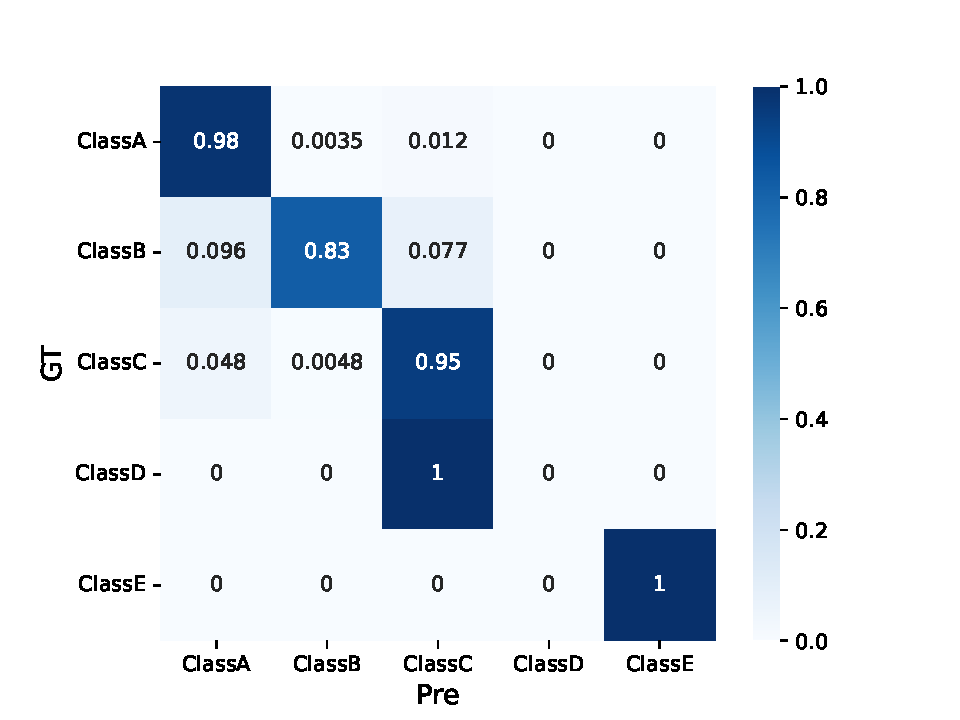
\includegraphics[keepaspectratio, scale=0.35]{images/deepimfam_confusion_matrix_ratio.pdf}
        \caption{増やす前}
      \end{minipage}
      \begin{minipage}[b]{0.45\linewidth}
        \centering
        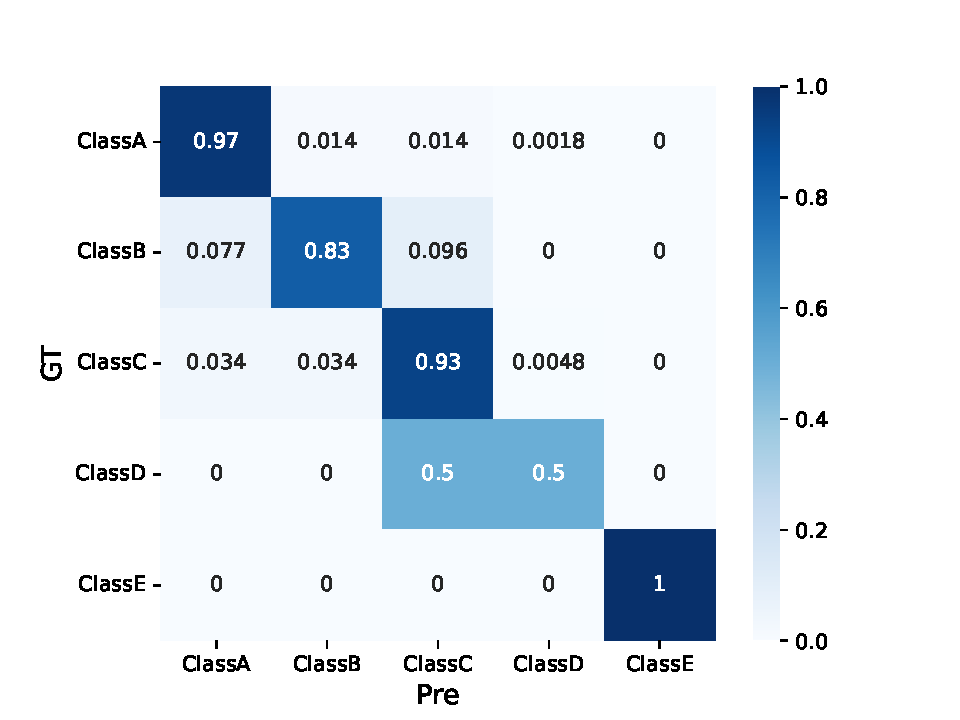
\includegraphics[keepaspectratio, scale=0.35]{images/deepimfam_augmentation_confusion_matrix_ratio.pdf}
        \caption{増やした後}
      \end{minipage}
    \end{figure}
  \end{frame}
  \begin{frame}{冬休み期間中行ったこと}
    \section{冬休み期間中行ったこと}
    \begin{itemize}
      \item コードの修正
      \item 卒論
      \begin{itemize}
        \item モデルに関する記述
        \item $F1_{score}$と計算結果の記述
      \end{itemize}
    \end{itemize}
  \end{frame}
\end{document}

